\section{Power}
\subsection{Power supply}

\todo[inline]{TBD voltage noise}
The 12V power can be connected either from AMC connector or from Stand alone power supply connected to Molex Connector(39-28-1043).

	\begin{figure}[htbp!]
		\centering
		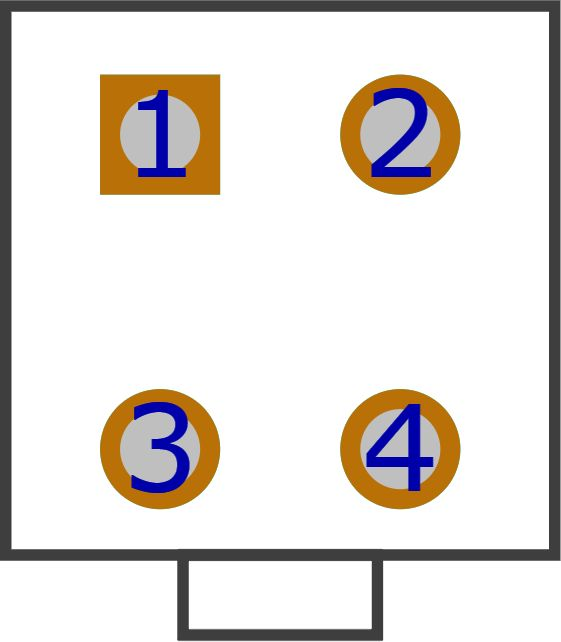
\includegraphics[scale=0.2]{img/molex.jpg}\\
		\caption{Power connector} 
	\end{figure}
\begin{center}
\begin{tabular}{|c|c|} \hline
	{\LARGE GND} & {\LARGE GND} \\ \hline
	{\LARGE +12} & {\LARGE +12} \\ \hline
\end{tabular}
\end{center}

Maximum board(AMC+RTM module) power consumption estimate to 3A @ 12V.\\

	\textit{\textbf{Note:} Please note that power consumption mostly depends from FPGA configuration. \\}

\begin{itemize}
 

\item Input voltage range: 10.8-13.2 [V]\\
\item The board needs active cooling. Approx. 20CFM in 20 C air.\\

\end{itemize}
\subsection{Power configuration} 

\subsubsection{Power map}


	\begin{figure}[htbp!]
		\centering
		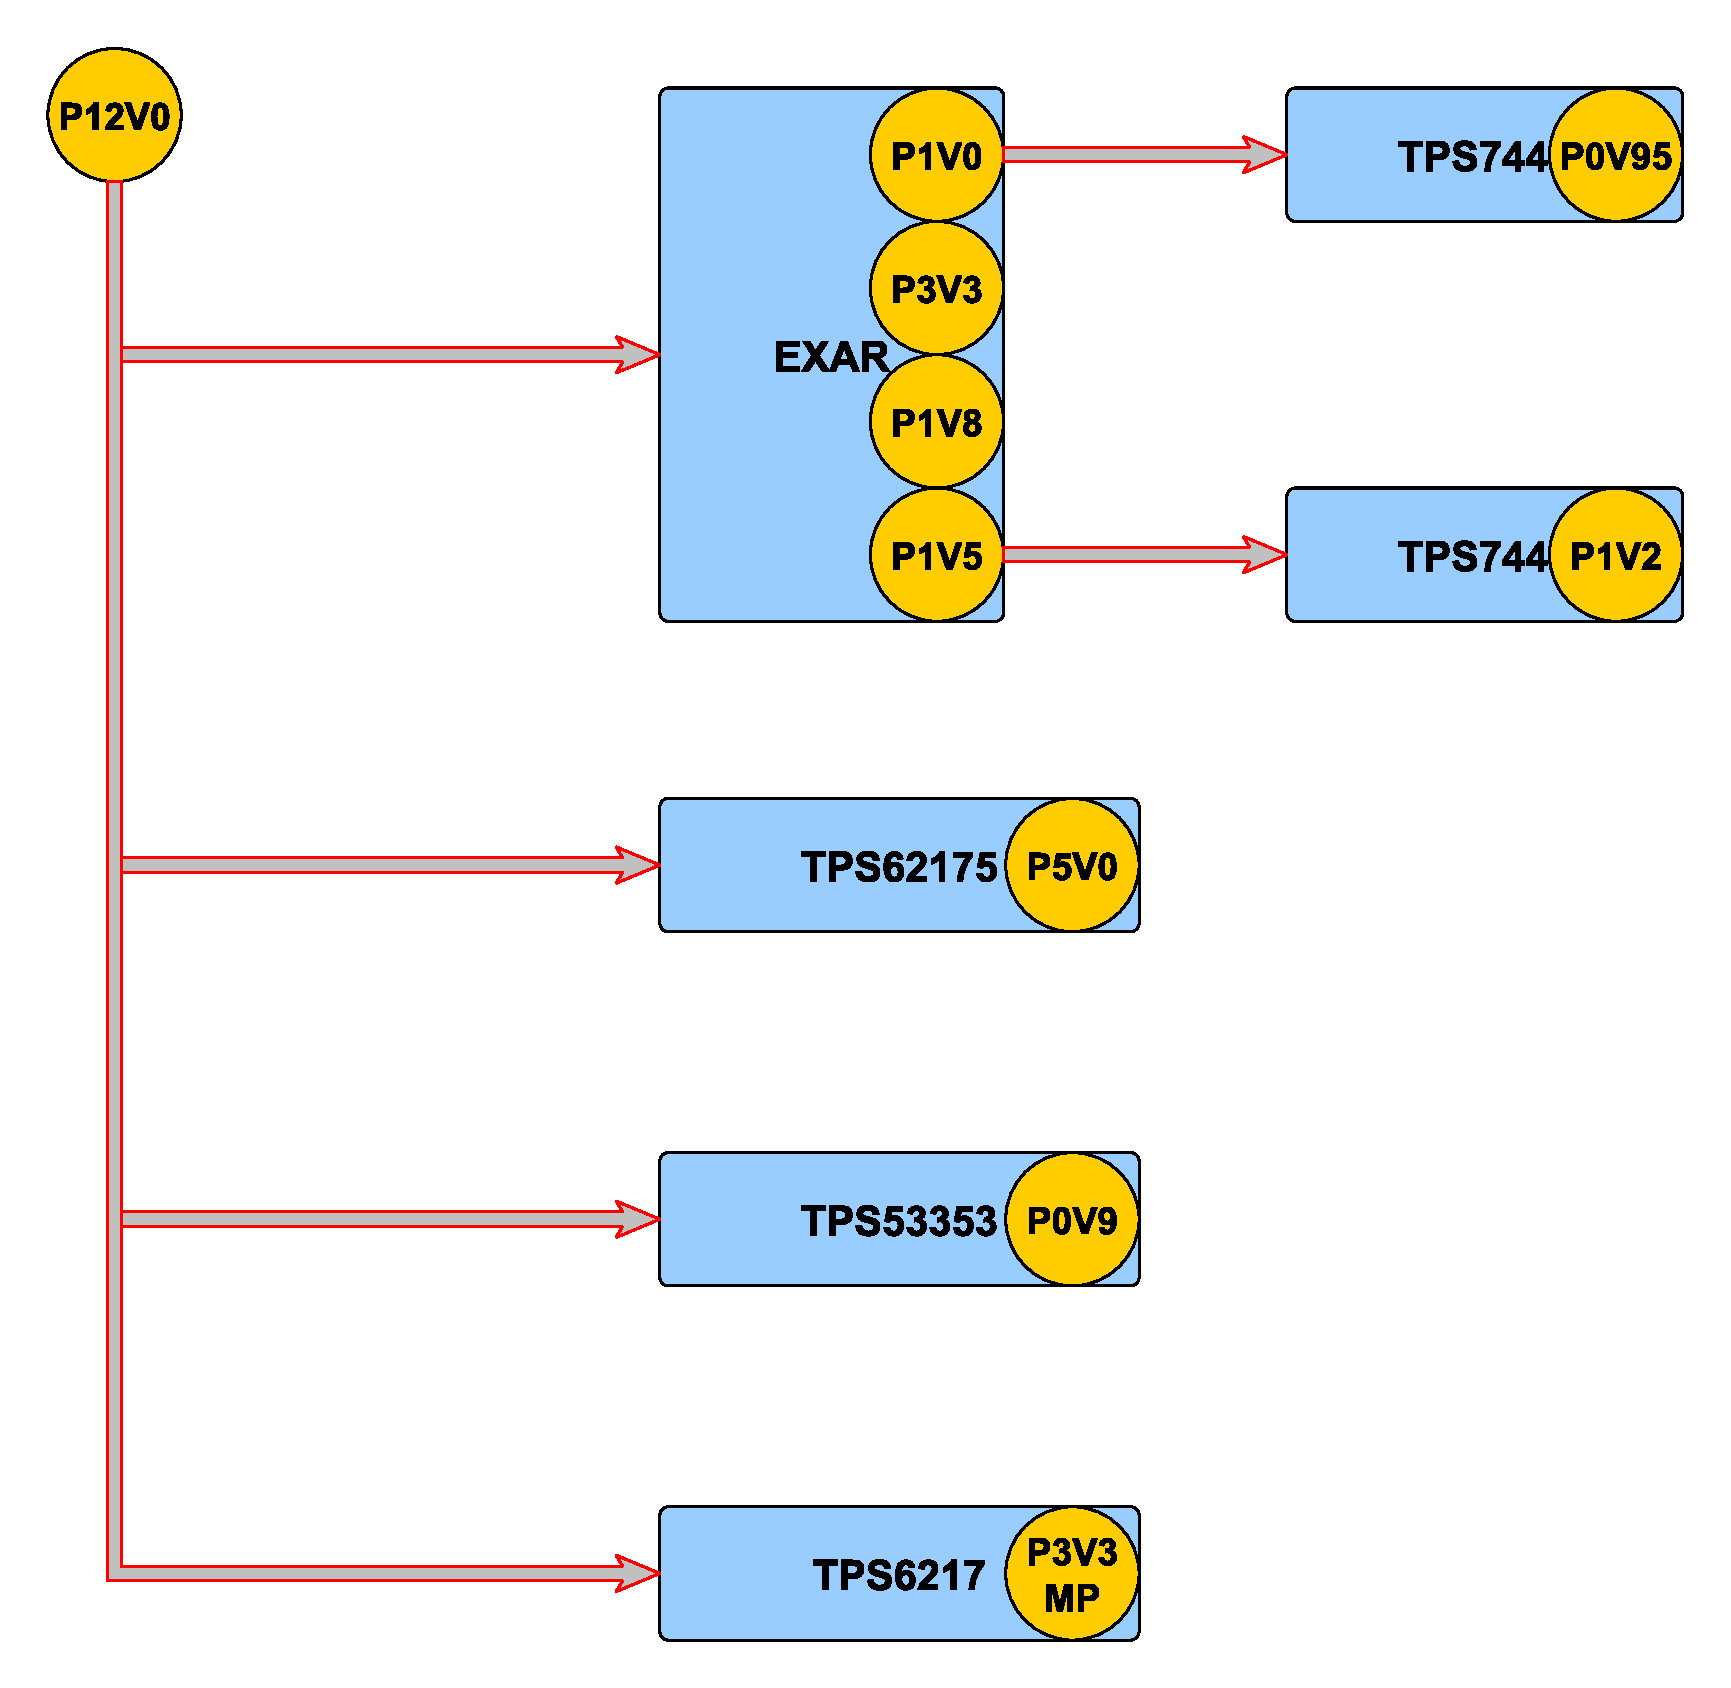
\includegraphics[scale=0.3]{img/pwr.eps}\\
		\caption{Power map} 
	\end{figure}
\clearpage	

\begin{longtable}{|c|c|c|} \hline
\multicolumn{3}{|c|}{voltages and currents}	\\ \hline
P0V9 & 0.9V & 10A \\ \hline
P0V95 & 0.95V & 31mA\\ \hline
P1V0 & 1.0V & 3A\\ \hline
P1V2 & 1.2V & 0.6A\\ \hline
P1V5 & 1.5V & 7.5A\\ \hline
P1V8 & 1.8V & 1.6A\\ \hline
P3V3 & 3.3 V & 2A\\ \hline
P3V3MP & 3.3V & 0.18A \\ \hline
P5V0 & 5.0V & 0.5A\\ \hline
\end{longtable}
	
\begin{longtable}{|c|c|c|} \hline
	\multicolumn{3}{|c|}{Maximum RTM voltages and currents}	\\ \hline
	P12V0 & 12V & 3A \\ \hline	
	P3V3MP\_RTM & 3.3V & 30mA \\ \hline
\end{longtable}
	
\subsubsection{Exar parameters}

Exar chip has 4 configurable outputs with configirable current limits. Channels 1, 3, 4 are power un on chip enable with 10ms delay. Channel 2 is power on 'EN\_PSU\_CH' signal. \\
%3V3 LDO is power on independently. \\

	\begin{figure}[htbp!]
		\centering
		\includegraphics[scale=0.6]{img/exar1.png}\\
		\caption{Exar configuration} 
	\end{figure}
	
	\begin{figure}[htbp!]
		\centering
		\includegraphics[scale=0.6]{img/exar2.png}\\
		\caption{Exar power on delays} 
	\end{figure}	
	
\clearpage	


\subsubsection{Exar configuration}
Exar chips are configured via I2C bus (MUX Port 5) or directly by connecting to W1 (call-out 28) header. For proper configuration \textbf{Exar Power Architect} in version \textbf{5.2-r1} is needed.
% Configuration files can be found at github in folder \href{https://github.com/m-labs/sinara/tree/master/EXAR\_config}{m-labs/sinara/Exar\_config}\\

\noindent
\textbf{Exar Power Archtect 5.2-r1:}
\href{https://www.exar.com/content/document.ashx?id=21632}{https://www.exar.com/content/document.ashx?id=21632}\\
\textbf{Configuration files:}
\href{https://github.com/m-labs/sinara/tree/master/EXAR\_config}{https://github.com/m-labs/sinara/tree/master/EXAR\_config}\\
\textbf{Datasheet:}\href{https://www.exar.com/ds/xr77129_1a_120514.pdf}{https://www.exar.com/ds/xr77129\_1a\_120514.pdf}\\
\textbf{Quick Start Guide:} \href{https://www.exar.com/files/powerxr/PA5-QSG_110_010614.pdf}{https://www.exar.com/files/powerxr/PA5-QSG\_110\_010614.pdf}\\


Actual voltages and current consumption, temperature can be found in Chip Dashboard. There is also oportunity to adjust settings.

	\begin{figure}[htbp!]
		\centering
		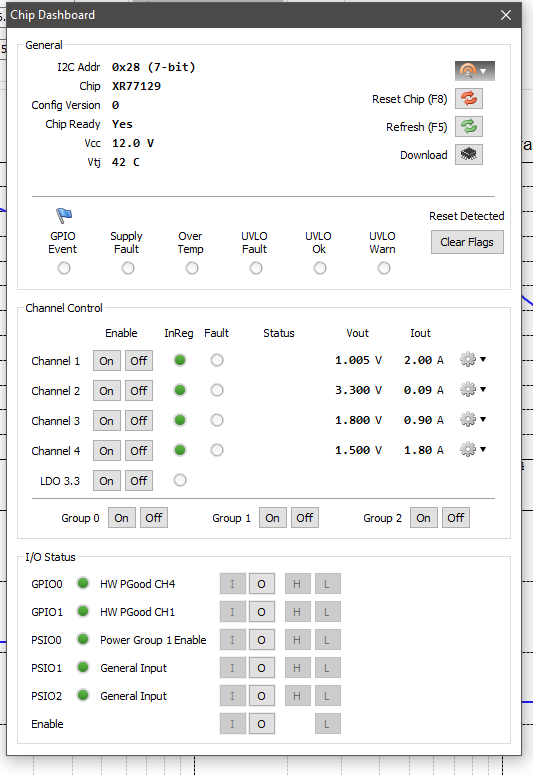
\includegraphics[scale=0.6]{img/exarprog.png}\\
		\caption{Chip Dashboard} 
	\end{figure}


